\documentclass[11pt, oneside]{article} 
\usepackage{geometry}
\geometry{letterpaper} 
\usepackage{graphicx}
	
\usepackage{amssymb}
\usepackage{amsmath}
\usepackage{parskip}
\usepackage{color}
\usepackage{hyperref}

\graphicspath{{/Users/telliott/Dropbox/Github-Math/geoproof/figures/}{/Users/telliott/Dropbox/Github-Math/figures/}}
% \begin{center} \includegraphics [scale=0.4] {gauss3.png} \end{center}

\title{Circles}
\date{}

\begin{document}
\maketitle
\Large

%[my-super-duper-separator]

\subsection*{Pi}

You undoubtedly know that the ratio of the circumference of a circle to its diameter is equal to the special value, $\pi$.
\begin{center} 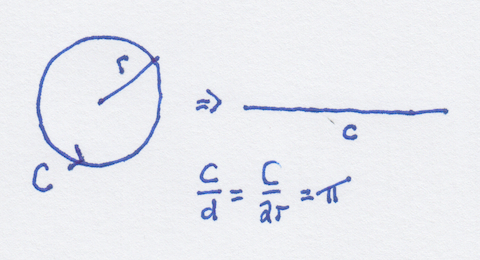
\includegraphics [scale=1.0] {H6.png} \end{center}
Since the diameter is twice the radius, we have that $C = 2 \pi r$.  This is true no matter how big or how small we make the circle.

It is amazing that the same constant $\pi$ is involved in the area of a circle.  The formula for area is 
\[ A = \pi r^2 \]
\begin{center} 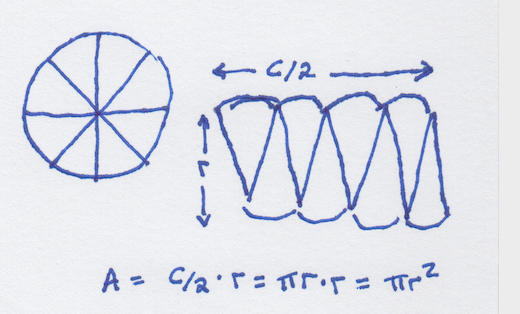
\includegraphics [scale=0.8] {H7.png} \end{center}
Above is a figure which makes this result seem reasonable.

Cut a circle into an even number of equal-sized slices and arrange them as shown on the right.  The height of the resulting rectangle-like figure is $r$ and the length of the combined top and bottom is $C$, so the width is $C/2 = \pi r$.  Using the rule for rectangles the area is
\[ C = \frac{C}{2} \cdot r = \pi r \cdot r = \pi r^2 \]

One simple thing to improve the estimate is to cut one of the end slices in half and add it to the other end.  That makes the end pieces vertical.  The other improvement is to cut the pizza into more slices.  This will have the effect of making the curvy edges straighter.  

Imagine if we just cut off the curved edges and ignored them.  The error will be significant with 8 pieces, but if the number of pieces is doubled, the error is more than halved.  Here's how it looks.  
\begin{center} 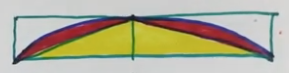
\includegraphics [scale=0.8] {H16.png} \end{center}
The error (underestimate for the area) for the whole sector is the yellow plus the red, that for the half-sector is just the red alone.  The latter is clearly less than half of the former, since there is less red than yellow.  Perhaps it is more like $1/3$.  So the total error obviously decreases as we make the curvy edges straighter by cutting the pizza into more slices.

\url{https://www.youtube.com/watch?v=R1HUtt2oo7A}

There is a subtle argument to make sure that we get all the way to the actual value.  But it looks persuasive, and in fact, it works.

\subsection*{one chord}

Draw any radius in a circle and the tangent where it meets the circle.  Then draw a chord that is parallel.
\begin{center} 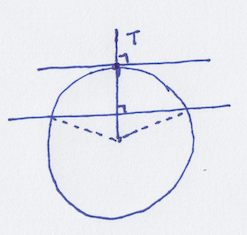
\includegraphics [scale=0.6] {H13.png} \end{center}
The radius cuts the chord in a right angle (because of the parallel construction).  This means that the two small triangles with parts of the chord and radii for sides are congruent (hypotenuse and a side plus a right angle).  So the chord is bisected.

Conversely, if we are given that the chord is bisected, then the two triangles are congruent by SSS.  So the angle where the radius cuts the chord is a right angle, which makes the chord parallel to the tangent drawn at the point where the radius meets the circle.

\subsection*{two chords}

Draw any two straight lines (called chords) in a circle.
\begin{center} 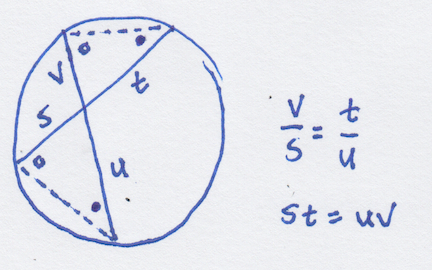
\includegraphics [scale=0.8] {H8.png} \end{center}

Recall the inscribed angle theorem.  The marked angles are peripheral angles that cut off the same arc from the circle.  By the theorem, they are equal, as marked.

This means that the two triangles are similar.  Ratios of similar sides give the result.
\[ \frac{v}{s}  = \frac{t}{u} \]
\[ st = uv \]
This is true for any two arcs of a circle.

Suppose we have two right angles inscribed into a circle along the same diameter.
\begin{center} 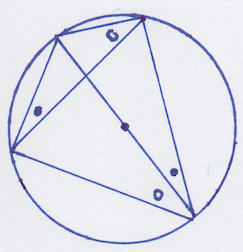
\includegraphics [scale=0.6] {T5.png} \end{center}
Below is a special case, where the dotted line forms right angles where it crosses the diameter.
\begin{center} 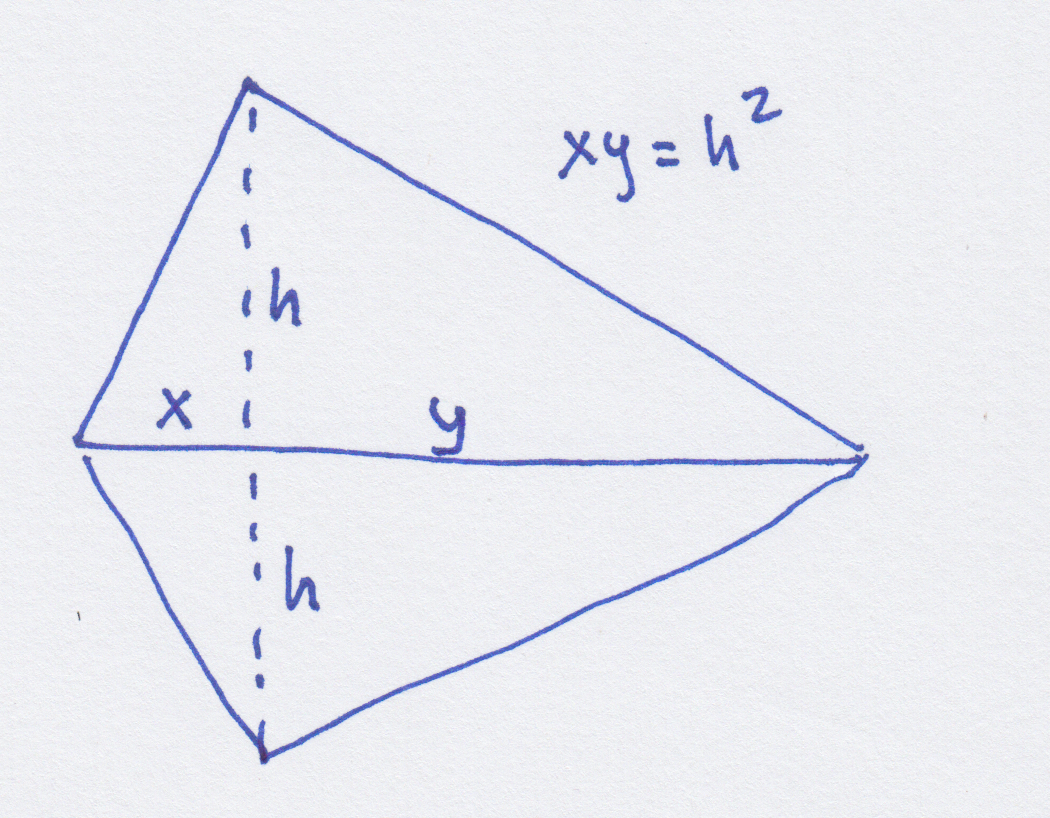
\includegraphics [scale=0.7] {H9b.png} \end{center}
Then, we have peripheral angles that subtend the same arc, so they are equal, and that gives similar right triangles.  We form the ratios:  $y/h = h/x$.

Alternatively, the result from above about chords means that
\[ xy = h^2 \]
Rearranging
\[ \frac{x}{h} = \frac{h}{y} \]
which means that the two smaller triangles are similar.  A third way we know this is from complementary angles.  We used it when we proved the Pythagorean theorem.

In the construction, we have the relationship $h = \sqrt{xy}$.  In statistics this is called the geometric mean of $x$ and $y$.  
\begin{center} 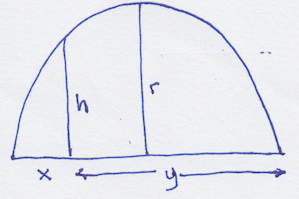
\includegraphics [scale=0.6] {H14.png} \end{center}
But we also have that $x + y = d = 2r$.  Hence $r = (x+y)/2$.  $r$ is the arithmetic mean of $x$ and $y$.  Imagine making $x$ larger and $y$ smaller or vice-versa.

The diagram shows that the arithmetic mean is always greater than the geometric mean, except when $x = y$.  Then, both are equal to $r$.

In the figure below, pick any two points in a circle and one exterior point and draw the triangle.  Also connect the points where the two sides we just drew intersect the circle, to form a smaller triangle.
\begin{center} 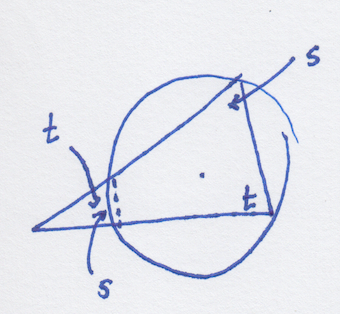
\includegraphics [scale=1.0] {H10.png} \end{center}
We have four points in a circle, forming a special four-sided figure called a cyclic quadrilateral.  In this figure, the opposing angles are supplementary, they add to 180.  This means the two angles $s$ are supplementary to the same angle.  The same is true of $t$.

Therefore we have two similar triangles.  So then we form the ratios of corresponding parts.
\begin{center} 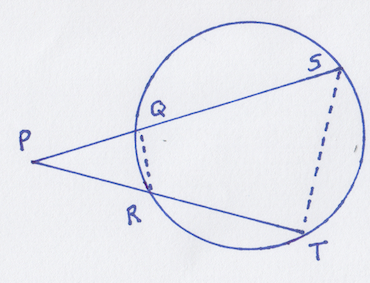
\includegraphics [scale=0.5] {H11.png} \end{center}
\[ \frac{PR}{PS} = \frac{PQ}{PT} \]
\[ PR \cdot PT = PQ \cdot PS \]

Finally, imagine that we slide the ends of the chord so that $S$ and $Q$ move toward each other, and finally meet at the tangent point.  Call the new point $S'$.  

$PS'$ is a tangent to the circle and
\[ {PS'}^2 = PR \cdot PT \]

Do the same thing on the other side, forming $PT'$.  Now
\[ {PS'}^2 = {PT'}^2 \]
\[ PS' = PT' \]

The two tangents drawn to a circle from any external point are equal.  Draw the two tangents, plus a line from the point to the center.  Form two congruent triangles (by side-hypotenuse in a right $\triangle$).  So $PT = PT'$.
\begin{center} 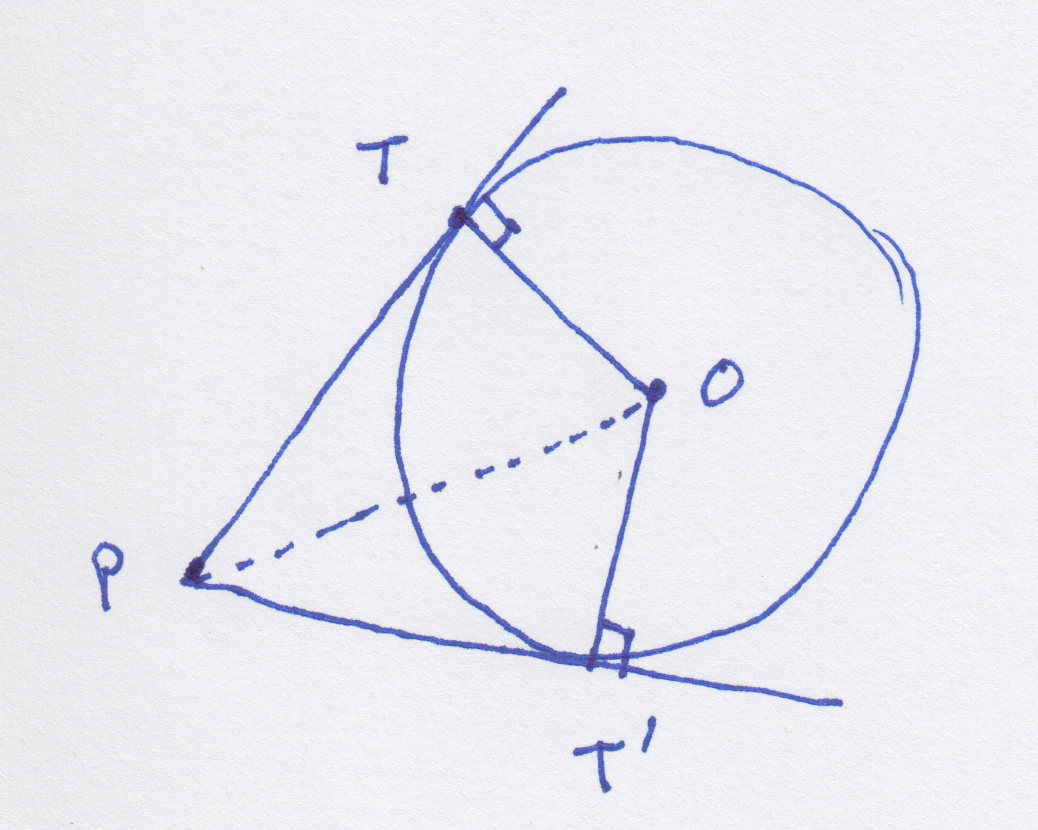
\includegraphics [scale=0.7] {H12.png} \end{center}

There is a circle that is just inscribed into a triangle, where each side is a tangent and just touches the circle.  It is called the incircle.
\begin{center} 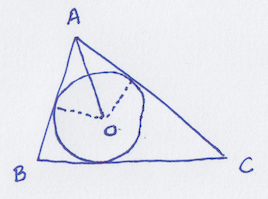
\includegraphics [scale=0.76] {H15.png} \end{center}

Draw $AO$ to form two triangles.  They are right triangles, because the sides are tangent.  Since they share a side and have a second side that is a radius, they are congruent.  Therefore $AO$ bisects $\angle A$.

Also, the distance from $A$ to the points of tangency is equal on both sides.  The tangents drawn from any exterior point to a circle are equal.  Call this distance $x$.  Then the combined area of these two triangles is just $rx$.  The total area of the triangle is $r(x + y + z)$ where $x + y + z$ is equal to the semi-perimeter of the triangle (one-half).

But the perimeter is the sum of the sides $a + b + c$.  So
\[ \triangle = r(x + y + z) = rs \]
where
\[ s = \frac{(a + b + c)}{2} \]


\end{document}
